%%%%%%%%%%%%%%%%%%%%%%%%%%%%%%%%%%%%%%%%%%%%%%%%%%%%%%%%%%%%%%%%%
%%% %
%%% % weiiszablon.tex
%%% % The Faculty of Electrical and Computer Engineering
%%% % Rzeszow University Of Technology diploma thesis Template
%%% % Szablon pracy dyplomowej Wydziału Elektrotechniki 
%%% % i Informatyki PRz
%%% % June, 2015
%%%%%%%%%%%%%%%%%%%%%%%%%%%%%%%%%%%%%%%%%%%%%%%%%%%%%%%%%%%%%%%%%
\documentclass[12pt]{article}

\usepackage{weiiszablon}

\author{Jakub Kusal}

% np. EF-123456, EN-654321, ...
\studentID{EF-169571}

\title{HuePi - aplikacja mobilna do obsługi żarówek Philips Hue}
\titleEN{HuePi - mobile app for managing Philips Hue bulbs}


%%% wybierz rodzaj pracy wpisując jeden z poniższych numerów: ...
% 1 = inżynierska	% BSc
% 2 = magisterska	% MSc
% 3 = doktorska		% PhD
%%% na miejsce zera w linijce poniżej
\newcommand{\rodzajPracyNo}{1}


%%% promotor
\supervisor{dr inż. Mariusz Mączka}
%% przykład: dr hab. inż. Józef Nowak, prof. PRz

%%% promotor ze stopniami naukowymi po angielsku
\supervisorEN{Mariusz Mączka, BEng, PhD}

\abstract{Treść streszczenia po polsku}
\abstractEN{Treść streszczenia po angielsku}

\begin{document}

% strona tytułowa
\maketitle

\blankpage

% spis treści
\tableofcontents

\clearpage
\blankpage


\section{Wstęp}
Używanie urządzeń typu \textit{Smart Home} cieszy się dziś coraz większym zainteresowaniem. \cite{popularność-smart-home} Nie jest to już
tylko ciekawostka technologiczna, która musi wiązać się z dużymi wydatkami.
Urządzenia tego typu stają się coraz bardziej przystępne cenowo, a producenci oferują coraz to większy wybór
samych urządzeń końcowych, jak i urządzeń integrujących całą resztę. Do takich urządzeń możemy zaliczyć m.in.:
kamery, zamki, głośniki, wyświetlacze, termostaty, gniazdka, żarówki itp. Widać więc, że spośród całej gamy urządzeń, mamy do wyboru opcje takie,
które pomagają zautomatyzować i wspomóc życie ludzi, jak również takie, które służą rozrywce.\\
Tym ostatnim typem urządzeń zajęto się w tym projekcie. Jego celem było stworzenie aplikacji mobilnej Android,
umożliwiającej sterowanie żarówkami producenta Philips, z serii Philips Hue.
Jest to cały ekosystem smart urządzeń, nie tylko żarówek. W jego skład wchodzą m.in. również:
paski LED, lampy stojące, lampki "choinkowe", przyciski, gniazdka, kamery, czujniki ruchu, czujniki zmierzchu.\\
Mimo ogromnej gamy urządzeń, można jednak zauważyć, iż nie występują w tym systemie żadnego rodzaju czujniki temperatury, czy sensory innych warunków atmosferycznych.
Tego typu akcesorium, mogłoby rozszerzyć, już jakże szeroki wachlarz możliwości ekosystemu Philips Hue, dzięki któremu korzystanie z np. żarówek stałoby się jeszcze bardziej ekscytujące.
Niniejszy projekt celuje w wypełnienie luki powstałej z faktu braku występowania wyżej wymienionych sensorów i przedstawienie konceptu, który pokazuje,
jak natywny ekosystem Philips Hue mógłby się rozwinąć.


\clearpage

\section{Cel oraz zakres projektu}
Celem projektu, było stworzenie aplikacji mobilnej na systemy operacyjne Android, przeznaczonej do sterowania żarówkami Philips Hue.
Nie stanowi ona pełnoprawnego oprogramowania do sterowania każdym produktem z ekosystemu Philips Hue.
Poza podstawowymi funkcjonalnościami, ma ona ukazać możliwości, o jakie możnaby rozszerzyć natywne ekosystemy Philips Hue.
Oprócz klasycznego sterowania, tj. ustawienie koloru, jasności, włączenia i wyłączenia, aplikacja miała umożliwiać wykorzystanie informacji o temperaturze,
w celu wyświetlania kolorów na podstawie tejże temperatury.


\subsection{Podobne oprogramowanie}
Pomysł na tego typu aplikację nie jest nowy. Istnieje wiele systemów, aplikacji i oprogramowania, które implementują funkcjonalności w zaprezentowanej tutaj aplikacji
i mają podobną filozofię. Przykłady niektórych z nich to:

\subsubsection{Philips Hue (aplikacja producenta)}
Philips Hue to oficjalna aplikacja mobilna producenta, przeznaczona głównie do zarządzania inteligentnym oświetleniem z rodziny Hue.
Udostępniana jest na urządzenia z systemem \textit{Android} oraz \textit{iOS},a jej podstawowym zadaniem jest umożliwienie pełnej konfiguracji i kontroli wszystkich elementów tego ekosystemu,
włącznie z tworzeniem scen, harmonogramów oraz automatyzacji.\\
Aplikacja komunikuje się z mostkiem Philips Hue, który jest fizycznym urządzeniem pełniącym rolę pośrednika pomiędzy oświetleniem a siecią lokalną.
Bezpośrednia integracja z mostkiem umożliwia:
\begin{itemize} \item dodawanie nowych żarówek lub innych akcesoriów (np. czujników ruchu, gniazdek) do ekosystemu,
	\item tworzenie i edytowanie tzw. \textit{scen świetlnych} (zestawów preferowanych ustawień światła, takich jak kolor, jasność czy temperatura barwowa),
	\item planowanie harmonogramów, pozwalających automatycznie włączać lub wyłączać światło o wybranych porach dnia,
	\item sterowanie głosowe (po odpowiedniej konfiguracji z asystentami pokroju Amazon Alexa, Apple Siri czy Google Assistant),
	\item konfigurowanie prostych reguł automatyzacji, które mogą reagować np. na wykrycie ruchu.
\end{itemize}
Korzystanie z aplikacji Philips Hue pozwala w łatwy sposób zapanować nad całym ekosystemem oświetlenia inteligentnego,
jednakże nie wspiera ona pomiaru parametrów środowiskowych, takich jak temperatura czy wilgotność.
W efekcie, choć zaspokaja większość typowych potrzeb związanych z inteligentnym oświetleniem,
nie rozszerza funkcjonalności systemu o dodatkowe odczyty czy też automatyzacje bazujące na czynnikach zewnętrznych (m.in. z użyciem czujników temperatury).

\subsubsection{Home Assistant}
Home Assistant to otwartoźródłowe oprogramowanie przeznaczone do lokalnego zarządzania i automatyzacji urządzeń w inteligentnym domu.
Można je wdrożyć zarówno na komputerach jednopłytkowych (np. Raspberry Pi), jak i na serwerach czy w środowisku kontenerowym (np. Docker).
Dzięki temu jest rozwiązaniem elastycznym pod względem wymagań sprzętowych i sposobu instalacji.\\
Dużą zaletą Home Assistant jest bogaty ekosystem integracji, który obejmuje również wsparcie
dla oświetlenia Philips Hue. Oprócz podstawowego sterowania, możliwe jest konfigurowanie zaawansowanych reguł automatyzacji,
reagujących np. na informacje z rozmaitych czujników (temperatury, wilgotności czy ruchu).
Platforma oferuje wbudowany edytor scen i skryptów, pozwalający na tworzenie wieloetapowych akcji wyzwalanych przez określone zdarzenia
(bądź harmonogramy czasowe).\\
Home Assistant zapewnia także dostęp do panelu webowego, dzięki któremu w wygodny sposób można zarządzać urządzeniami,
przeglądać ich status, a także dostosowywać interfejs użytkownika zgodnie z własnymi preferencjami.
Ze względu na swoją otwartość i rozbudowaną społeczność, umożliwia wprowadzanie dodatkowych wtyczek (\textit{add-ons})
i komponentów, co sprawia, że możliwości systemu są praktycznie nieograniczone.
Duża liczba gotowych rozwiązań udostępnianych w formie repozytoriów społecznościowych pozwala
szybko uruchamiać nowe funkcjonalności lub modyfikować istniejące.

\subsubsection{Google Home}
Google Home to platforma i aplikacja mobilna rozwijana przez firmę Google, służąca do zarządzania urządzeniami inteligentnego domu.
W odróżnieniu od rozwiązań stricte samodzielnych, aplikacja ta ściśle integruje się z ekosystemem usług Google oraz asystentem głosowym Google Assistant,
co pozwala sterować wieloma sprzętami za pomocą komend głosowych.\\
Podobnie jak inne rozwiązania z tej kategorii, Google Home obsługuje oświetlenie Philips Hue, umożliwiając jego konfigurację, tworzenie tzw. pokoi (ang. \textit{rooms})
i grupowanie urządzeń w praktyczny sposób. Pozwala także w prosty sposób zaprogramować podstawowe sceny świetlne czy harmonogramy włączania i wyłączania.
Ze względu na powiązania z kontem Google, cała konfiguracja pozostaje dostępna z różnych urządzeń (smartfon, tablet, głośniki Nest itp.),
co ułatwia zdalne sterowanie oświetleniem oraz innymi elementami inteligentnego domu (np. termostatami, głośnikami czy kamerami).\\
W przeciwieństwie do bardziej zaawansowanych platform otwartoźródłowych, Google Home koncentruje się głównie na wygodzie i prostocie użytkowania.
Oferuje co prawda możliwość definiowania automatyzacji – tzw. \textit{Routines} – jednak nie pozwala na tak rozbudowane scenariusze integracji,
jak systemy pokroju Home Assistant. Niemniej jednak dzięki swojemu podejściu „wszystko w jednym” i ścisłemu powiązaniu z usługami Google,
Google Home jest dobrym wyborem dla użytkowników szukających łatwego w konfiguracji i intuicyjnego rozwiązania do codziennego sterowania oświetleniem Philips Hue,
jak również innymi urządzeniami typu \textit{Smart Home}.

\clearpage

\section{Wykorzystany sprzęt i technologie}
Projekt można podzielić na 2 główne części: serwer uruchomiony na Raspberry Pi 3B wraz z czujnikiem oraz aplikacja moblina.
\subsection{Serwer na Raspberry Pi}

\subsubsection{Raspberry Pi 3B}
Raspberry Pi 3B to komputer jednopłytkowy opracowany przez fundację Raspberry Pi, który od momentu wprowadzenia na rynek zdobył ogromną popularność zarówno wśród hobbystów,
jak i profesjonalistów. Jego niewielkie wymiary (85.6 mm x 56.5 mm) oraz niska cena sprawiają,
że stanowi doskonałe rozwiązanie do tworzenia różnorodnych projektów technologicznych, takich jak systemy \textit{Smart Home},
urządzenia IoT (Internet of Things), serwery multimedialne, a nawet jako komputer edukacyjny.
Raspberry Pi 3B jest wyposażony w czterordzeniowy procesor ARM Cortex-A53 o taktowaniu 1.2 GHz, co w połączeniu z 1 GB pamięci RAM
pozwala na płynne działanie lekkich systemów operacyjnych, takich jak Raspberry Pi OS, Ubuntu czy inne dystrybucje Linuxa zoptymalizowane pod kątem architektury ARM.
Wbudowana karta Wi-Fi obsługująca standard 802.11n oraz moduł Bluetooth 4.1 umożliwiają bezprzewodową komunikację z innymi urządzeniami
oraz sieciami lokalnymi bez konieczności stosowania dodatkowych adapterów.\\
Płyta oferuje liczne interfejsy wejścia i wyjścia, co czyni ją wyjątkowo wszechstronną w zastosowaniach praktycznych. Na wyposażeniu znajdują się m.in.:
\begin{itemize}
    \item 40-pinowy złącze GPIO (\textit{General Purpose Input/Output}), które umożliwia podłączanie i sterowanie szeroką gamą urządzeń peryferyjnych,
	takich jak czujniki, diody LED, przyciski czy serwomechanizmy,
    \item 4 porty USB 2.0, umożliwiające podłączenie akcesoriów takich jak klawiatura, mysz, kamera czy pendrive,
    \item złącze HDMI do podłączenia monitora, co pozwala na wykorzystanie urządzenia jako miniaturowego komputera stacjonarnego,
    \item złącze CSI do kamer i DSI do ekranów, co otwiera możliwości budowy systemów monitoringu czy interaktywnych wyświetlaczy,
    \item interfejsy komunikacyjne, takie jak \textit{I\textsuperscript{2}C}, \textit{SPI} i \textit{UART}, służące do komunikacji z różnymi modułami i sensorami.
\end{itemize}
Jednym z przykładów modułów, które mogą być zintegrowane z Raspberry Pi 3B, jest czujnik BME280. Urządzenie to umożliwia precyzyjne pomiary temperatury,
wilgotności oraz ciśnienia atmosferycznego. Dzięki swoim kompaktowym wymiarom i wsparciu dla interfejsu \textit{I\textsuperscript{2}C},
czujnik BME280 jest często wykorzystywany w projektach związanych z monitorowaniem warunków środowiskowych, systemami \textit{Smart Home}
czy urządzeniami prognozującymi pogodę. Raspberry Pi 3B, w połączeniu z takim czujnikiem, może odczytywać dane w czasie rzeczywistym,
co pozwala na ich dalsze przetwarzanie oraz wykorzystanie w aplikacjach automatyzacji lub raportowania. Dzięki wielu dostępnym bibliotekom,
integracja czujnika z urządzeniem jest stosunkowo prosta i szybka.\\
Raspberry Pi 3B wspiera również wiele oprogramowania pozwalającego na wygodną integrację z urządzeniami \textit{Smart Home}.
Na przykład, instalacja platform takich jak poprzednio omawiany Home Assistant umożliwia tworzenie zaawansowanych reguł automatyzacji
oraz centralne zarządzanie wieloma urządzeniami, w tym oświetleniem Philips Hue. Możliwość uruchamiania serwerów lokalnych (np. HTTP czy MQTT) sprawia,
że Raspberry Pi może pełnić rolę centrum sterowania lub bramy komunikacyjnej w bardziej rozbudowanych projektach.\\
Dzięki aktywnej społeczności użytkowników, Raspberry Pi 3B jest dobrze udokumentowany, a w sieci dostępne są liczne poradniki i przykłady implementacji projektów.
Wszechstronność i niska cena tego komputera sprawiają, że jest on chętnie wybierany zarówno do celów edukacyjnych, jak i komercyjnych.
Raspberry Pi 3B może być zatem kluczowym elementem projektów opartych na inteligentnym oświetleniu, takich jak \textit{HuePi},
w których służy jako serwer API przetwarzający dane z sensorów oraz komunikujący się z żarówkami w ekosystemie Philips Hue.


\subsubsection{Czujnik BME280}
Czujnik BME280 to wielofunkcyjny sensor środowiskowy opracowany przez firmę Bosch, przeznaczony do pomiaru trzech podstawowych parametrów:
temperatury, wilgotności oraz ciśnienia atmosferycznego. Ze względu na swoją wszechstronność, kompaktowe rozmiary oraz wysoką precyzję pomiarów,
znajduje szerokie zastosowanie w projektach związanych z automatyką domową, Internetem Rzeczy (IoT) oraz urządzeniami monitorującymi warunki środowiskowe.\\
BME280 wspiera interfejsy komunikacyjne \textit{I\textsuperscript{2}C} oraz \textit{SPI}, co czyni go łatwym do integracji z różnymi mikrokontrolerami i komputerami jednopłytkowymi,
takimi jak Raspberry Pi. Dzięki temu użytkownik ma dużą elastyczność w wyborze platformy sprzętowej. Czujnik charakteryzuje się niskim zużyciem energii,
co sprawia, że idealnie nadaje się do zastosowań w systemach zasilanych bateryjnie.\\
Specyfikacja czujnika obejmuje:
\begin{itemize}
    \item Zakres pomiaru temperatury: od -40°C do +85°C, z dokładnością do ±1°C\cite{bme280-datasheet},
    \item Zakres pomiaru wilgotności: od 0\% do 100\% RH (wilgotność względna), z dokładnością ±3\% RH\cite{bme280-datasheet},
    \item Zakres pomiaru ciśnienia atmosferycznego: od 300 hPa do 1100 hPa, z dokładnością do ±1 hPa\cite{bme280-datasheet}.
\end{itemize}
Czujnik jest wykorzystywany w aplikacjach takich jak:
\begin{itemize}
    \item monitorowanie warunków środowiskowych w budynkach (np. wilgotność w pomieszczeniach mieszkalnych),
    \item systemy pogodowe, w tym prognozowanie zmian ciśnienia,
    \item automatyzacja domowa, np. w połączeniu z systemami sterowania oświetleniem, które mogą reagować na zmiany temperatury,
    \item urządzenia IoT, zbierające dane do analizy i przesyłające je do systemów chmurowych lub lokalnych serwerów.
\end{itemize}
Czujnik BME280 jest często wykorzystywany w projektach prototypowych i edukacyjnych dzięki szerokiej dostępności bibliotek programistycznych.
Możliwość dokładnych pomiarów w połączeniu z łatwością integracji sprawia, że czujnik ten idealnie nadaje się do implementacji w projektach
takich jak \textit{HuePi}, w których dane np. o temperaturze mogą być przetwarzane w celu dostosowania funkcji systemu, np. sterowania oświetleniem.

\subsubsection{FastAPI}
FastAPI to nowoczesny framework do tworzenia aplikacji webowych oraz API w języku Python. Został zaprojektowany z myślą o wysokiej wydajności,
prostocie użytkowania oraz integracji z typowaniem statycznym w Pythonie. Dzięki zastosowaniu standardu ASGI (Asynchronous Server Gateway Interface),
FastAPI wspiera obsługę zapytań w trybie asynchronicznym, co czyni go szczególnie przydatnym w aplikacjach wymagających dużej liczby jednoczesnych zapytań
lub intensywnej komunikacji z zewnętrznymi usługami.
FastAPI jest oparty na narzędziu \textit{Starlette} (do obsługi zapytań i trasowania) oraz \textit{Pydantic} (do walidacji i serializacji danych).
Oferuje funkcjonalności, które czynią go jednym z najpopularniejszych frameworków do budowy API, takich jak:
\begin{itemize}
    \item Automatyczne generowanie dokumentacji API na podstawie definicji punktów końcowych (\textit{endpoints}) i typów danych.
	Dokumentacja jest dostępna w formatach \textit{Swagger UI} oraz \textit{ReDoc}, co ułatwia testowanie i integrację API.
    \item Wsparcie dla typowania w Pythonie, co umożliwia precyzyjne określenie wejściowych i wyjściowych danych dla punktów końcowych.
	Typowanie pozwala również na automatyczną walidację danych i zmniejsza ryzyko błędów programistycznych.
    \item Obsługa asynchroniczności dzięki natywnemu wsparciu dla konstrukcji \texttt{async} i \texttt{await}, co sprawia,
	że framework doskonale sprawdza się w aplikacjach wymagających współbieżności, takich jak przetwarzanie danych w czasie rzeczywistym czy obsługa mikroserwisów.
    \item Łatwa integracja z systemami autoryzacji i uwierzytelniania, np. przy użyciu protokołów OAuth2 czy JWT (\textit{JSON Web Tokens}).
    \item Rozbudowane wsparcie dla operacji związanych z przetwarzaniem żądań HTTP, takich jak pobieranie danych z parametrów,
	nagłówków czy plików przesyłanych przez użytkowników.
\end{itemize}
FastAPI znajduje zastosowanie w wielu obszarach, takich jak:
\begin{itemize}
    \item Tworzenie mikroserwisów – dzięki asynchroniczności i wysokiej wydajności framework świetnie nadaje się do budowy modułowych aplikacji o niewielkiej złożoności.
    \item Systemy IoT – FastAPI może być używane jako interfejs do komunikacji między urządzeniami a centralnym serwerem.
    \item Tworzenie RESTful API – pozwala na szybkie i efektywne tworzenie punktów końcowych dla aplikacji webowych czy mobilnych.
    \item Integracja z systemami ML/AI – FastAPI jest często wykorzystywane do udostępniania modeli uczenia maszynowego w formie usług API,
	umożliwiających ich łatwą integrację z innymi aplikacjami.
\end{itemize}
Dzięki intuicyjnej składni, bogatej dokumentacji oraz dużej społeczności użytkowników, FastAPI stał się jednym z najchętniej wybieranych narzędzi
do budowy nowoczesnych aplikacji webowych i API w Pythonie.

\subsection{Aplikacja mobilna}

\subsubsection{Język Kotlin}
Kotlin to nowoczesny, wieloplatformowy język programowania opracowany przez firmę JetBrains. Jego pierwsza stabilna wersja została wydana w 2016 roku \cite{kotlin-data-wydania},
a już w 2017 roku został oficjalnie ogłoszony przez Google jako język wspierany do tworzenia aplikacji na system Android.
Kotlin został zaprojektowany jako nowoczesna alternatywa dla Javy, oferująca większą produktywność, czytelność kodu oraz nowoczesne funkcje,
które redukują ryzyko błędów programistycznych.\\
Kotlin jest językiem zorientowanym obiektowo z elementami programowania funkcyjnego. Wyróżnia go pełna interoperacyjność z kodem napisanym w Javie,
co umożliwia łatwą migrację istniejących projektów. Dzięki temu programiści mogą stopniowo wprowadzać Kotlin do swoich aplikacji,
korzystając z bibliotek i narzędzi napisanych w Javie.\\
Jednym z kluczowych powodów popularyzacji Kotlina jest fakt, że Google wymaga jego użycia do pracy z Jetpack Compose – nowoczesnym narzędziem
do tworzenia interfejsów użytkownika w aplikacjach na system Android. Dzięki Jetpack Compose, aplikacje mogą być projektowane szybciej i w bardziej intuicyjny sposób,
co sprawia, że Kotlin staje się praktycznie nieodzownym elementem ekosystemu Android.\\
Do najważniejszych cech języka Kotlin należą:
\begin{itemize}
    \item \textbf{Bezpieczeństwo typów} – Kotlin eliminuje ryzyko wystąpienia błędów typu \texttt{NullPointerException} dzięki systemowi \textit{nullable types},
	który wymaga jawnego oznaczenia zmiennych mogących przechowywać wartość \texttt{null}.
    \item \textbf{Krótszy i czytelniejszy kod} – Kotlin wprowadza nowoczesne konstrukcje składniowe, takie jak wyrażenia lambda, funkcje rozszerzające czy destrukturyzacja,
	co znacząco zmniejsza ilość kodu wymaganego do implementacji określonych funkcji w porównaniu z Javą.
    \item \textbf{Wsparcie dla programowania funkcyjnego} – język umożliwia tworzenie wyrażeń lambda, operacje na kolekcjach oraz wykorzystanie funkcji wyższego rzędu,
	co zwiększa elastyczność kodu.
    \item \textbf{Pełna kompatybilność z JVM} – Kotlin działa na maszynie wirtualnej Javy (\textit{Java Virtual Machine}) i może wykorzystywać
	wszystkie istniejące biblioteki oraz frameworki napisane w Javie.
    \item \textbf{Obsługa współbieżności} – Kotlin wprowadza natywne wsparcie dla współbieżności w postaci \textit{coroutines},
	które umożliwiają łatwiejsze i bardziej efektywne zarządzanie współbieżnymi zadaniami.
    \item \textbf{Wieloplatformowość} – dzięki Kotlin Multiplatform język pozwala na tworzenie wspólnego kodu, który może działać na różnych platformach,
	takich jak Android, iOS, JVM, JavaScript, a nawet natywne aplikacje desktopowe.
\end{itemize}
Kotlin znajduje zastosowanie w wielu dziedzinach:
\begin{itemize}
    \item \textbf{Tworzenie aplikacji mobilnych} – Kotlin jest obecnie najpopularniejszym językiem do tworzenia aplikacji na system Android dzięki swojej prostocie,
	wydajności i wsparciu przez Google.
    \item \textbf{Tworzenie aplikacji serwerowych} – Kotlin może być używany z frameworkami takimi jak Ktor czy Spring Boot do budowy nowoczesnych API i aplikacji webowych.
    \item \textbf{Programowanie wieloplatformowe} – Kotlin Multiplatform umożliwia tworzenie wspólnego kodu, który działa zarówno na systemach Android, jak i iOS,
	co znacząco obniża koszty i czas rozwoju aplikacji.
    \item \textbf{Aplikacje desktopowe} – dzięki Kotlin/Native można tworzyć aplikacje działające na systemach operacyjnych takich jak Windows, macOS czy Linux.
\end{itemize}
Kotlin zdobył uznanie wśród programistów dzięki swojej nowoczesności, elastyczności i możliwościom. Używa go ponad 60\% profesjonalnych programistów Android.
\cite{kotlin-popularność} Jego integracja z narzędziami JetBrains, takimi jak IntelliJ IDEA, oraz wsparcie przez Google sprawiają, że jest to język przyszłościowy,
szczególnie w kontekście tworzenia aplikacji mobilnych.

\subsubsection{Jetpack Compose}
Jetpack Compose to nowoczesny framework opracowany przez Google, służący do tworzenia interfejsów użytkownika (\textit{UI}) w aplikacjach na system Android.
Jest to narzędzie oparte na deklaratywnym podejściu do budowy interfejsów, które pozwala tworzyć dynamiczne i złożone układy w sposób bardziej intuicyjny i efektywny
niż tradycyjne podejście z wykorzystaniem XML.\\
Jednym z kluczowych wymagań do pracy z Jetpack Compose jest użycie języka Kotlin, który dzięki swojej nowoczesnej składni i wsparciu dla programowania funkcyjnego
doskonale współgra z deklaratywnym stylem tworzenia interfejsów. Jetpack Compose integruje się bezpośrednio z istniejącym ekosystemem Androida,
co umożliwia stopniową migrację aplikacji opartych na tradycyjnych układach XML.
Do najważniejszych cech Jetpack Compose należą:
\begin{itemize}
    \item \textbf{Deklaratywne podejście} – interfejsy są definiowane jako funkcje w języku Kotlin, co pozwala na proste i czytelne opisywanie widoków oraz ich zależności.
    \item \textbf{Reaktywność} – framework automatycznie odświeża interfejs użytkownika w odpowiedzi na zmiany w stanie aplikacji,
	co eliminuje potrzebę ręcznego zarządzania aktualizacjami widoków.
    \item \textbf{Komponenty wielokrotnego użytku} – Jetpack Compose oferuje bibliotekę gotowych komponentów, takich jak przyciski, pola tekstowe czy listy,
	które można łatwo dostosowywać do potrzeb projektu.
    \item \textbf{Integracja z Jetpack} – Compose współpracuje z innymi bibliotekami wchodzącymi w skład ekosystemu Jetpack, takimi jak
	\textit{Navigation}, \textit{LiveData} czy \textit{ViewModel}, co ułatwia zarządzanie stanem aplikacji i nawigacją.
    \item \textbf{Obsługa wieloplatformowa} – Jetpack Compose jest rozwijany także w wersji \textit{Compose Multiplatform},
	co umożliwia tworzenie interfejsów użytkownika nie tylko dla Androida, ale również dla innych platform, takich jak \textit{desktop} czy przeglądarki internetowe.
    \item \textbf{Szybka iteracja} – dzięki funkcji \textit{hot reload} programiści mogą natychmiast zobaczyć efekty wprowadzonych zmian w kodzie interfejsu, co znacznie przyspiesza proces tworzenia aplikacji.
\end{itemize}
Jetpack Compose rozwiązuje wiele problemów związanych z tradycyjnym tworzeniem interfejsów w Androidzie,takich jak skomplikowane zarządzanie układami w XML
czy konieczność ręcznego obsługiwania zmian w widokach. Umożliwia budowanie nowoczesnych i estetycznych interfejsów przy jednoczesnym zmniejszeniu ilości kodu
oraz uproszczeniu procesu tworzenia aplikacji.\\
W porównaniu z tradycyjnym podejściem opartym na Javie i XML, Jetpack Compose w połączeniu z językiem Kotlin oferuje znacznie większą produktywność i przejrzystość kodu.
W Kotlinie deklaratywne definiowanie interfejsów pozwala uniknąć zbędnego kodu „klejącego” (tzw. \textit{boilerplate code}), który był często niezbędny w Javie
do wiązania widoków XML z logiką aplikacji. Kotlin wprowadza funkcje rozszerzające, lambdy i programowanie funkcyjne, co czyni kod bardziej zwięzłym i łatwiejszym w utrzymaniu.
Jetpack Compose całkowicie eliminuje potrzebę używania XML, upraszczając proces tworzenia złożonych interfejsów i redukując możliwość wystąpienia błędów związanych
z niezgodnością kodu XML i logiki w Javie. Dzięki tym cechom Jetpack Compose i Kotlin razem redefiniują sposób budowania aplikacji na Androida,
kładąc nacisk na nowoczesność, elastyczność i szybkość tworzenia oprogramowania.

\subsubsection{DataStore Preferences}
DataStore Preferences to nowoczesna biblioteka Android Jetpack opracowana przez Google, służąca do przechowywania niewielkich ilości danych w sposób wydajny,
bezpieczny i zgodny z zasadami programowania asynchronicznego. Stanowi następcę starszego mechanizmu \textit{SharedPreferences}, eliminując wiele jego ograniczeń,
takich jak synchroniczność i ryzyko blokowania głównego wątku (\textit{UI thread}).\\
Biblioteka DataStore oferuje dwa tryby przechowywania danych:
\begin{itemize}
    \item \textbf{Preferences DataStore} – przeznaczone do przechowywania prostych danych w formacie klucz-wartość, podobnie jak \textit{SharedPreferences}.
    \item \textbf{Proto DataStore} – pozwalające na przechowywanie bardziej złożonych struktur danych przy użyciu protokołu Protobuf
	(zalecane w przypadku bardziej rozbudowanych wymagań dotyczących danych).
\end{itemize}
Główne cechy DataStore Preferences to:
\begin{itemize}
    \item \textbf{Asynchroniczność} – operacje zapisu i odczytu danych są wykonywane asynchronicznie przy użyciu Kotlin Coroutines,
	co zapobiega blokowaniu wątku głównego i poprawia wydajność aplikacji.
    \item \textbf{Reaktywność} – dane są dostępne jako strumienie \textit{Flow}, dzięki czemu można je obserwować i automatycznie reagować na ich zmiany
	w czasie rzeczywistym.
    \item \textbf{Bezpieczeństwo typów} – dzięki jawnemu definiowaniu typów danych, DataStore zmniejsza ryzyko błędów związanych z niezgodnością typów,
	co było częstym problemem w \textit{SharedPreferences}.
    \item \textbf{Prosta implementacja} – DataStore Preferences wykorzystuje intuicyjne API i jest w pełni zintegrowane z ekosystemem Android Jetpack, co umożliwia łatwą integrację z innymi komponentami, takimi jak ViewModel czy LiveData.
\end{itemize}

\subsubsection*{Przykłady użycia DataStore Preferences}
\noindent \textbf{Zapis danych:} Dane są przechowywane w pliku konfiguracyjnym w sposób asynchroniczny i bezpieczny:
\begin{lstlisting}[language=Kotlin]
suspend fun savePreference(key: Preferences.Key<String>, value: String) {
    dataStore.edit { preferences ->
        preferences[key] = value
    }
}
\end{lstlisting}

\noindent \textbf{Odczyt danych:} Dane są dostępne jako strumień \textit{Flow}, co umożliwia ich obserwację w czasie rzeczywistym:
\begin{lstlisting}[language=Kotlin]
val preferenceFlow: Flow<String?> = dataStore.data.map { preferences ->
    preferences[PreferencesKeys.SOME_KEY]
}
\end{lstlisting}

\subsubsection*{Zastosowania DataStore Preferences}
\noindent DataStore Preferences jest idealnym rozwiązaniem do przechowywania niewielkich ustawień aplikacji, takich jak:
\begin{itemize}
    \item preferencje użytkownika, np. ustawienia motywu (ciemny/jasny),
    \item preferencje językowe aplikacji,
    \item zapamiętywanie stanu aplikacji, np. ostatnio wybranej zakładki.
\end{itemize}

\subsubsection*{Porównanie z SharedPreferences}
\noindent DataStore Preferences oferuje wiele usprawnień w porównaniu z \textit{SharedPreferences}:
\begin{itemize}
    \item Operacje są wykonywane asynchronicznie, co zapobiega przycinaniu interfejsu użytkownika podczas zapisu lub odczytu danych.
    \item Dzięki wykorzystaniu strumieni \textit{Flow}, DataStore umożliwia automatyczne reagowanie na zmiany danych w czasie rzeczywistym, podczas gdy \textit{SharedPreferences} wymagało ręcznej aktualizacji widoków.
    \item DataStore Preferences wspiera nowoczesne podejście do programowania z użyciem Kotlin Coroutines, co czyni go bardziej zgodnym z nowoczesnymi standardami tworzenia aplikacji na Androida.
\end{itemize}
DataStore Preferences to nowoczesne i wydajne narzędzie do przechowywania danych w aplikacjach Android,które eliminuje ograniczenia starszych rozwiązań,
takich jak \textit{SharedPreferences}. Dzięki asynchroniczności, reaktywności i bezpieczeństwu typów, DataStore Preferences pozwala tworzyć bardziej wydajne
i stabilne aplikacje, które lepiej spełniają wymagania współczesnych użytkowników.

\subsubsection{Biblioteka Retrofit}
Retrofit to nowoczesna biblioteka open-source opracowana przez firmę Square, która służy do komunikacji z serwerami RESTful poprzez wykonywanie żądań HTTP.
Retrofit ułatwia integrację aplikacji Android z zewnętrznymi API, zapewniając prosty i wydajny sposób na wykonywanie zapytań sieciowych oraz przetwarzanie ich odpowiedzi.\\
Główną zaletą biblioteki Retrofit jest jego modułowość i łatwość w użyciu. Biblioteka automatyzuje wiele aspektów komunikacji sieciowej, takich jak serializacja
i deserializacja danych, obsługa różnych typów żądań HTTP (\texttt{GET}, \texttt{POST}, \texttt{PUT}, \texttt{DELETE}) oraz zarządzanie nagłówkami i parametrami zapytań.

\subsubsection*{Cechy biblioteki Retrofit}
\begin{itemize}
    \item \textbf{Automatyczna konwersja danych} – Retrofit obsługuje różne formaty danych, takie jak JSON czy XML, przy użyciu adapterów serializujących (np. Gson, Moshi). Konwersja danych wejściowych i wyjściowych jest w pełni zautomatyzowana.
    \item \textbf{Obsługa interfejsów} – zapytania sieciowe są definiowane w postaci interfejsów, co pozwala na przejrzysty i modularny kod.
    \item \textbf{Łatwe konfigurowanie} – Retrofit umożliwia łatwe zarządzanie podstawowymi ustawieniami żądań, takimi jak adres bazowy serwera, nagłówki czy parametry.
    \item \textbf{Obsługa asynchroniczności} – Retrofit wspiera natywną obsługę Kotlin Coroutines i \texttt{RxJava}, co umożliwia asynchroniczne wykonywanie zapytań bez blokowania głównego wątku.
    \item \textbf{Rozszerzalność} – biblioteka pozwala na łatwe dodawanie własnych adapterów do obsługi niestandardowych typów danych.
\end{itemize}

\subsubsection*{Przykłady użycia}
\textbf{Definiowanie interfejsu API:}
\begin{lstlisting}[language=Kotlin]
import retrofit2.http.GET
import retrofit2.http.Path

interface ApiService {
	@GET("users/{id}")
	suspend fun getUser(@Path("id") userId: Int): User
}
\end{lstlisting}

\textbf{Tworzenie instancji Retrofit:}
\begin{lstlisting}[language=Kotlin]
import retrofit2.Retrofit
import retrofit2.converter.gson.GsonConverterFactory

val retrofit = Retrofit.Builder()
	.baseUrl("https://api.example.com/")
	.addConverterFactory(GsonConverterFactory.create())
	.build()

val apiService: ApiService = retrofit.create(ApiService::class.java)
\end{lstlisting}

\textbf{Wykonywanie zapytań:}
\begin{lstlisting}[language=Kotlin]
import kotlinx.coroutines.CoroutineScope
import kotlinx.coroutines.Dispatchers
import kotlinx.coroutines.launch

CoroutineScope(Dispatchers.IO).launch {
	try {
		val user = apiService.getUser(1)
		// Przetwarzanie odpowiedzi
		println("User: ${user.name}")
	} catch (e: Exception) {
		e.printStackTrace()
	}
}
\end{lstlisting}

\subsubsection*{Zastosowania biblioteki Retrofit}
\noindent Retrofit jest szeroko stosowany w aplikacjach Android do:
\begin{itemize}
    \item komunikacji z API RESTful, np. pobierania danych użytkownika, postów czy obrazów,
    \item przesyłania danych w aplikacjach korzystających z zapytań \texttt{POST} lub \texttt{PUT},
    \item integracji aplikacji z zewnętrznymi serwisami, takimi jak usługi pogodowe, mapy czy systemy płatności.
\end{itemize}

\subsubsection*{Zalety biblioteki Retrofit w porównaniu z innymi rozwiązaniami}
\noindent W porównaniu z tradycyjnym mechanizmem \texttt{HttpURLConnection} czy biblioteką \texttt{Volley}, Retrofit oferuje większą modularność,
automatyzację przetwarzania danych oraz wsparcie dla nowoczesnych narzędzi, takich jak Kotlin Coroutines. Dzięki temu programiści mogą znacznie szybciej
i łatwiej integrować aplikacje Android z zewnętrznymi usługami sieciowymi, tworząc przy tym kod bardziej przejrzysty i łatwy w utrzymaniu.

\clearpage


\subsubsection{Rysunki i tabele} \label{Subsec:Rysunki-i-tabele}
Tekst podstawowy w tabeli pisze się czcionką o rozmiarze 10 punktów, pojedyncza interlinia. Dane liczbowe – wyśrodkowane, dane tekstowe – wyrównane do lewej. Rysunki i tabele zamieszcza się wyśrodkowane na stronie, bez wcięcia pierwszego wiersza.

W akapicie poprzedzającym rysunek lub tabelę musi znajdować się krótki opis, czego dotyczy dany rysunek/tabela (odniesienie do rysunku/tabeli). Tytuły numeruje się zgodnie z kolejnością w danym rozdziale: numer\_rozdziału.numer\_tabeli/rysunku (np. rys. 2.1, tabela 3.5). W tytule rysunku/tabeli, zaczerpniętych z literatury, podaje się odnośnik do właściwej pozycji. Należy zadbać o to, aby opisy na rysunkach były czytelne (czcionka 8 punktów lub większa). Staraj się nie wymuszać numeracji, pozwól aby robił to za ciebie \LaTeX. Stosuj \verb!\label! do znakowania obiektów, do których być może w tekście się będziesz odwoływał (rozdziały, rysunki, tabele, wzory, listingi \ldots). Odwołuj się do nich w tekście  za pomocą funkcji \verb!\ref{NazwaObiektu}!. Pamiętaj, że \LaTeX\, korzystając z polecenia \verb|latex| nie odczytuje z plików .jpg, .png ich wielkości. Polecenie \verb|latex| generuje plik \verb|DVI|. Jeżeli chcesz go używać zgłosi stosowny błąd. Aby się go pozbyć zdefiniuj wielkość natywną pliku grafiki. Polecamy jednak używanie zamiast polecenia \verb|latex|, polecenie \verb|pdflatex|, wówczas problem nie wystąpi.\\

\begin{example}
	[\ldots] co umożliwia wyznaczenie wartości napięcia. Na rys. \ref{Fig:schemat} przedstawiono schemat obwodu z równolegle dołączoną pojemnością $C_p$.
\end{example}

\begin{figure}[ht]
	\centering
	\includegraphics[width=6cm]{figures/fig1.png}
	\caption{Tytuł rysunku, rozmiar 11 pkt., pojedyncza interlinia, akapit wyśrodkowany, bez wcięcia pierwszego wiersza. Na końcu tytułu rysunku/tabeli nie stawia się kropki [8]}
	\label{Fig:schemat}
\end{figure}

\begin{example}
	[\ldots] Na rysunku \ref{Fig:wykres} pokazano przykładową zależność prądów pasmowych $i_\mathrm{ph}$ bezszczotkowego silnika prądu stałego z magnesami trwałymi w funkcji położenia wirnika $\theta$.
\end{example}

\begin{figure}[ht]
	\centering
	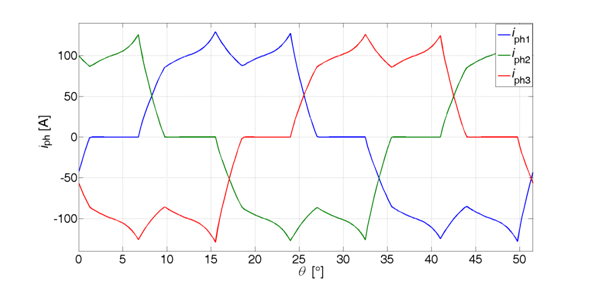
\includegraphics[width=12cm]{figures/fig2.png}
	\caption{Tytuł rysunku, rozmiar 11 pkt., pojedyncza interlinia, akapit wyśrodkowany, bez wcięcia pierwszego wiersza. Na końcu tytułu rysunku/tabeli nie stawia się kropki [8]}
	\label{Fig:wykres}
\end{figure}


\begin{example}
	[\ldots] oraz indukcyjności wzajemnej. W tabeli \ref{Tab:tabela} przedstawiono podstawowe parametry obwodu nieliniowego, zasilanego napięciem trójfazowym.
\end{example}

\begin{table}[ht]
	\caption{Tytuł tabeli, rozmiar 11 pkt., pojedyncza interlinia, akapit wyrównany do lewej}
	\centering
	\begin{tabular}{|c|c|c|c|c|}
		\hline
		$U$ [V] & $I$ [mA] & $R$, [k$\Omega$] & $L$ [mH] & $R/R_{20}$ \\
		\hline
		13,6    & 7,29     & 3,94             & 100      & 1,25       \\
		\hline
	\end{tabular}

	\label{Tab:tabela}
\end{table}

{\subsubsection{Listingi programów}}

W pracy dyplomowej możesz umieszczać fragmenty programów. Pamiętaj, aby umieszczać krótkie, tylko najważniejsze fragmenty kodów źródłowych. Zawsze je komentuj w treści
pracy dyplomowej. Typowo w \LaTeX\ kody źródłowe umieszczane są w środowisku verbatim (\verb|\begin{verbatim}...\end{verbatim}|). Obecnie instnieje jednak bardziej nowoczesne i bardziej funkcjonalne środowisko \verb|lstlisting| (wymaga zainstalowanego w systemie pakietu \verb|listings|). Zwróć uwagę, że możesz kolorować składnię
automatycznie za pomocą parametru \verb|language|. W niniejszym dokumencie przedstawiono dwa przykłady listingów, Listing \ref{KodMatlab1} to przykład kodu źródłowego Matlaba, a poniżej Listing \ref{KodPerl1} dla Perl'a.\\
%\komentarz{

\begin{lstlisting}[language=Matlab,caption=Listing programu Matlab,label={KodMatlab1}]
i = 1
p = 3
for i = 1:10
    if i > 3
        i=i+p
    else 
        i=i+1
    end
end
\end{lstlisting}

\begin{lstlisting}[language=Perl,caption=Listing programu Perl,label={KodPerl1}]
  my $url ='http://pei.prz.edu.pl';
  use LWP::Simple;
  my $content = get $url;
  die "Couldn't get $url" unless defined $content;
  print $content;
  print "\n";
  print "Length " + length($content)
\end{lstlisting}

Z pewnością przeglądając źródło tego dokumentu zobaczysz, że kody źródłowe powinny mieć zdefiniowane parametry \verb|label|, aby łatwo w tekście do nich się odwoływać.
Numeracja linii jest w stylu domyślnie włączona (to przydatne, bo w treści pracy łatwo odwołać się dzięki temu do konkretnego wiersza w kodzie źródłowym), możesz je wyłączyć podając jako parametr \verb|numbers=none|. Więcej szczegółów możesz odnaleźć w sekcji \verb|\lstset| pliku arkusza styli.
%}


\subsubsection{Numerowanie i punktowanie}

\begin{enumerate}[label=\arabic*), leftmargin=1.25cm]
	\item Pierwszy poziom (stosuje się numerowanie lub punktowanie). Formatowanie:
	      akapit wyjustowany, wcięcie od lewej 0,75 cm, wysunięcie co 0,5 cm.
	\item Znakiem numerowania jest liczba (z kropką lub nawiasem).
	      \begin{itemize}[label=-,labelsep=0.4cm,leftmargin=0.6cm]
		      \item drugi poziom (stosuje się wyłącznie punktowanie). Formatowanie: akapit
		            wyjustowany, wcięcie od lewej 1,25 cm, wysunięcie co 0,5 cm,
		      \item znakiem punktowania jest łącznik lub mała litera alfabetu (z nawiasem). Nie
		            zaleca się stosowania kropek, strzałek itp.,
		      \item punktowane akapity rozpoczyna się minuskułą (małą literą), na końcu akapitu
		            stawia się przecinek, ostatni punktowany akapit kończy się kropką.
	      \end{itemize}
	\item Numerowane akapity rozpoczyna się majuskułą (wielką literą) i kończy kropką.
	\item Należy zwrócić uwagę, aby nie rozdzielać numerowania/punktowania pomiędzy
	      kolejnymi stronami tekstu.
\end{enumerate}


\subsection{Wykaz literatury}

W wykazie literatury zamieszcza się wyłącznie pozycje, na które powołano się
w pracy. Kolejność numerów w wykazie – zgodna z kolejnością pojawiania się danej
pozycji w tekście.

Format akapitu: akapit wyjustowany, wysunięcie 0,75 cm. Prawidłowo opracowany
wykaz został zaprezentowany w niniejszym dokumencie w odpowiednim rozdziale, oznaczonym jako „Literatura”  (pozycja nr \cite{str} to zasoby internetowe,
\cite{Jakubczyk1997} – książka, \cite{Barski2011} – artykuł w czasopiśmie, \cite{dokum} – karta katalogowa).

	{\subsection{Wydruk pracy}}

Przed wydrukiem należy usunąć ewentualne błędy literowe i sprawdzić prawidłową
interpunkcję. Przykładowo, łącznik zapisuje się za pomocą krótkiego minusa (np.
badawczo-rozwojowy) natomiast myślnik -- stosowany w zdaniach wtrąconych -- zapisuje
się za pomocą długiej pauzy. Dzielenie wyrazów według uznania Autora (można podzielić
długie wyrazy, powodujące duże „rozstrzelenie” tekstu w poprzedzającym wierszu. Zaleca się usunięcie pojedynczych znaków na końcu wiersza oraz podwójnych spacji w tekście.
Dla przedrostka „mikro” należy unikać stosowania litery „u” zamiast „$\mu$”. Znak „$\mu$” można
otrzymać przytrzymując lewy Alt i wpisując na klawiaturze numerycznej 0181 (podobnie
„stopień”: Alt-0176). W celu uniknięcia „rozstrzelenia” liczb i ich jednostek zaleca się
używanie „twardej” spacji pomiędzy liczbą i jednostką. Należy sprawdzić, czy tytuły
podrozdziałów/zakresów nie zostały jako pojedyncze wiersze na poprzedniej stronie oraz
czy rysunki/tabele i ich tytuły nie zostały rozdzielone pomiędzy kolejnymi stronami.

Pracę drukuje się dwustronnie. Zaleca się wydruk w kolorze. Przed wydrukiem
należy ponumerować strony (czcionka 10 pkt., dół strony, akapit wyśrodkowany). Strony
tytułowej oraz strony z podziękowaniem nie numeruje się. Spis treści rozpoczyna się od
strony numer 3 (lub 5, jeżeli zamieszczono podziękowania).

\clearpage

\section{Podsumowanie i wnioski końcowe}

1 $\div$ 3 stron merytorycznie podsumowanie najważniejszych elementów pracy oraz wnioski wynikające z osiągniętego celu pracy. Proponowane zalecenia i modyfikacje oraz rozwiązania będące wynikiem realizowanej pracy.

Ostatni akapit podsumowania musi zawierać wykaz własnej pracy dyplomanta i zaczynać się od sformułowania: „Autor za własny wkład pracy uważa: \ldots”.

\clearpage

\section*{Załączniki}
\addcontentsline{toc}{section}{Załączniki}

Według potrzeb zawarte i uporządkowane uzupełnienie pracy o dowolny materiał źródłowy (wydruk programu komputerowego, dokumentacja kons\-truk\-cyj\-no-\-tech\-no\-lo\-gicz\-na, konstrukcja modelu -- makiety -- urządzenia, instrukcja obsługi urządzenia lub stanowiska laboratoryjnego, zestawienie wyników pomiarów i obliczeń, informacyjne materiały katalogowe itp.).


\clearpage

\addcontentsline{toc}{section}{Literatura}

\begin{thebibliography}{4}
	\bibitem{popularność-smart-home} https://www.statista.com/forecasts/887613/number-of-smart-homes-in-the-smart-home-market-in-the-world
	\bibitem{bme280-datasheet} https://www.mouser.com/datasheet/2/783/BST-BME280-DS002-1509607.pdf
	\bibitem{kotlin-data-wydania} https://kotlinlang.org/docs/faq.html
	\bibitem{kotlin-popularność} https://developer.android.com/kotlin
	\bibitem{Jakubczyk1997} Jakubczyk T., Klette A.: Pomiary w akustyce. WNT, Warszawa 1997.
	\bibitem{Barski2011} Barski S.: Modele transmitancji. Elektronika praktyczna, nr 7/2011, str. 15-18.
	\bibitem{dokum} Czujnik S200. Dokumentacja techniczno-ruchowa. Lumel, Zielona Góra, 2001.
	\bibitem{Pawluk2001} Pawluk K.: Jak pisać teksty techniczne poprawnie, Wiadomości Elektrotechniczne, Nr 12, 2001, str. 513-515.
\end{thebibliography}

\clearpage

\makesummary

\end{document}
